\chapter{DroneControl}

\section{Introductie} \label{sec:initiele_planning}

In dit hoofdstuk zal besproken worden op welke manier de drone softwarematig wordt aangestuurd.

\subsection{Ontwerpkeuzes}

Het eerste waarover een beslissing moest genomen worden was het al dan niet gebruiken van een reeds bestaande framework, en zoja welke. Bij de keuze van drone werd beschikbaarheid van documentatie reeds in het achterhoofd gehouden waardoor er veel opties beschikbaar waren. Volgende opties werden onderzocht:

\begin{itemize}
\item python-ardrone
\item YADrone
\item AR Drone Simulink Development-Kit
\item AR Drone Toolkit for LabVIEW
\item Nodecopter
\item Parrot SDK
\end{itemize}

Er werd al snel besloten om gebruik te maken van een framework, aangezien er hierdoor meer tijd kan gestoken worden in de eigenlijke projectdoelstellingen. De meeste frameworks vielen ook al meteen af aangezien ze niet voldoende gedocumenteerd waren of gebruik maakten van software en/of programmeertaal waarmee we niet voldoende vertrouwd waren. De laatste keuze moest gemaakt worden tussen de python framework en Nodecopter. Doorslaggevend voor de keuze voor Nodecopter was de zeer grote beschikbaarheid van documentatie en extra modules. Aangezien er via Python werd gecommuniceerd zorgde dit er wel voor dat de droneControl moest worden opgesplitst in twee delen. Eenerzijds het Nodejs deel dat de commando's doorstuurt naar de drone, en anderzijds het python script dat de positie zal ophalen van de mqqt server. Tot slot moest er nog besloten worden in welk van de twee delen de positie verwerkt zou worden naar een commando dat doorgegeven kan worden aan de drone. Hiervoor is python gekozen aangezien we hier meer ervaring mee hebben.




\section{Communiceren met de drone via Nodecopter}


Aangezien alle berekeningen reeds worden gedaan in het Python script is de node kant niet veel meer dan een tussenstuk dat alle data ontvangt op een lokale socket en direct doorstuurt naar de drone door middel van Nodecopter commands. Het enige andere nog vernoemenswaardige feature is dat het script ook de hoogte zal ontvangen van de drone en dit terugsturen over dezelfde socket. Dit gebeurd parallel aan de besturingslus zodanig deze niet moet staan wachten op niet triviale hoogte data.\\

We gebruiken de 'node-ar-library' van Nodecopter. Dit is de standaard library voor het besturen van de drone. Deze laat toe om de drone high level aan de sturen. Er kan simpelweg een drone object worden aangemaakt waarop functies als 'forward' of 'left' kunnen opgeroepen worden met als argumenten een fractionele snelheid tussen 0 (stil) en 1 (maximum snelheid). Voor andere richtingen in het 3-dimensioneel vlak bestaan gelijkaardige commands. Rotatie gebeurt ook gelijkaardig, met een hoeksnelheid tussen -1 en 1.\\

Het gebruik van de 'ardrone-autonomy' library werd ook onderzocht. Dit is een uitbreiding op de standaar library die toelaat om de drone nog meer high level aan te sturen aan de hand van afstand en draaihoek in plaats van snelheid. Als snel werd echter duidelijk dat voor binnenvluchten met kleinere foutmarges deze library niet accuraat genoeg is. Dit komt doordat de drone geen ingebouwde gps heeft, en zijn relatieve positie dus enkel maar kan baseren op het geleverde vermogen aan de motoren, wat verre van accuraat is.



\begin{figure}[h]
\caption{Een flowchart van het Nodescript}
\centering
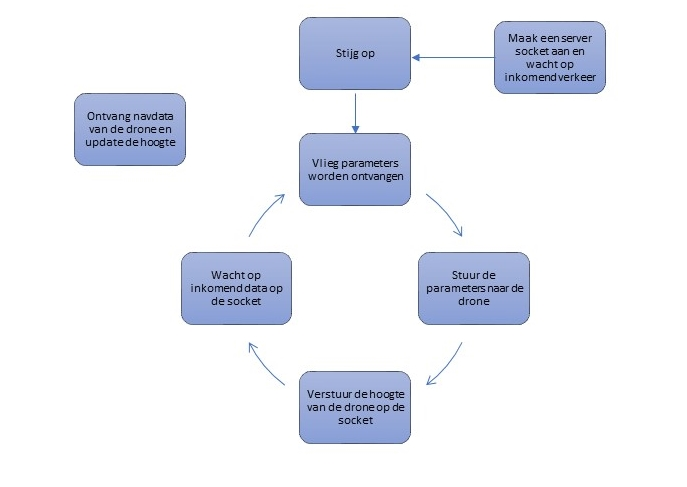
\includegraphics[width=\textwidth]{images/node_server_flowchart}
\end{figure}

\section{Verwerken van de data in Python}


